%!TEX root = TIHSC_Project_main.tex
\chapter{System synthesis}
System synthesis is part of the model-based system design approach where it is used obtain a transaction level model from a system specification, as seen in figure \ref{fig:modelBasedSyn}. 

\begin{figure}[H]
\centering
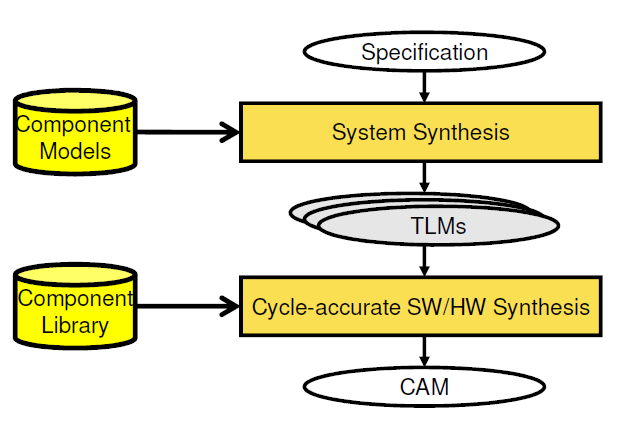
\includegraphics[scale=0.5]{modelBasedSynthesis}
\caption{Model bases synthesis}
\label{fig:modelBasedSyn}
\end{figure}

The system behavioural model from figure \ref{fig:SpecificationModel} in section \ref{cha:sysBehMod} describes the specification for a Texton mapping system. 
The processes, channels and memory variables from the specification model is used as input to the different steps of the system synthesis.  

\section{Allocation}
The first step of system synthesis is allocation of the needed hardware components. 
The processes of the specification model suggest the need for at least one CPU to handle reading and writing of the image. 
All the processes could be run on a single CPU, however given requirement \ref{req:timeReq} which states that the Texton filtering should be done within a minute, is it unlikely that a single CPU can make it in time. 
Therefore a hardware IP block is allocated to support the CPU with the computation-heavy processes.
\\Figure \ref{fig:SpecificationModel} also shows that processes P2 and P3 depend on a memory variable, which is allocated as a memory component. 

\section{Binding}

\begin{figure}[H]
1\centering
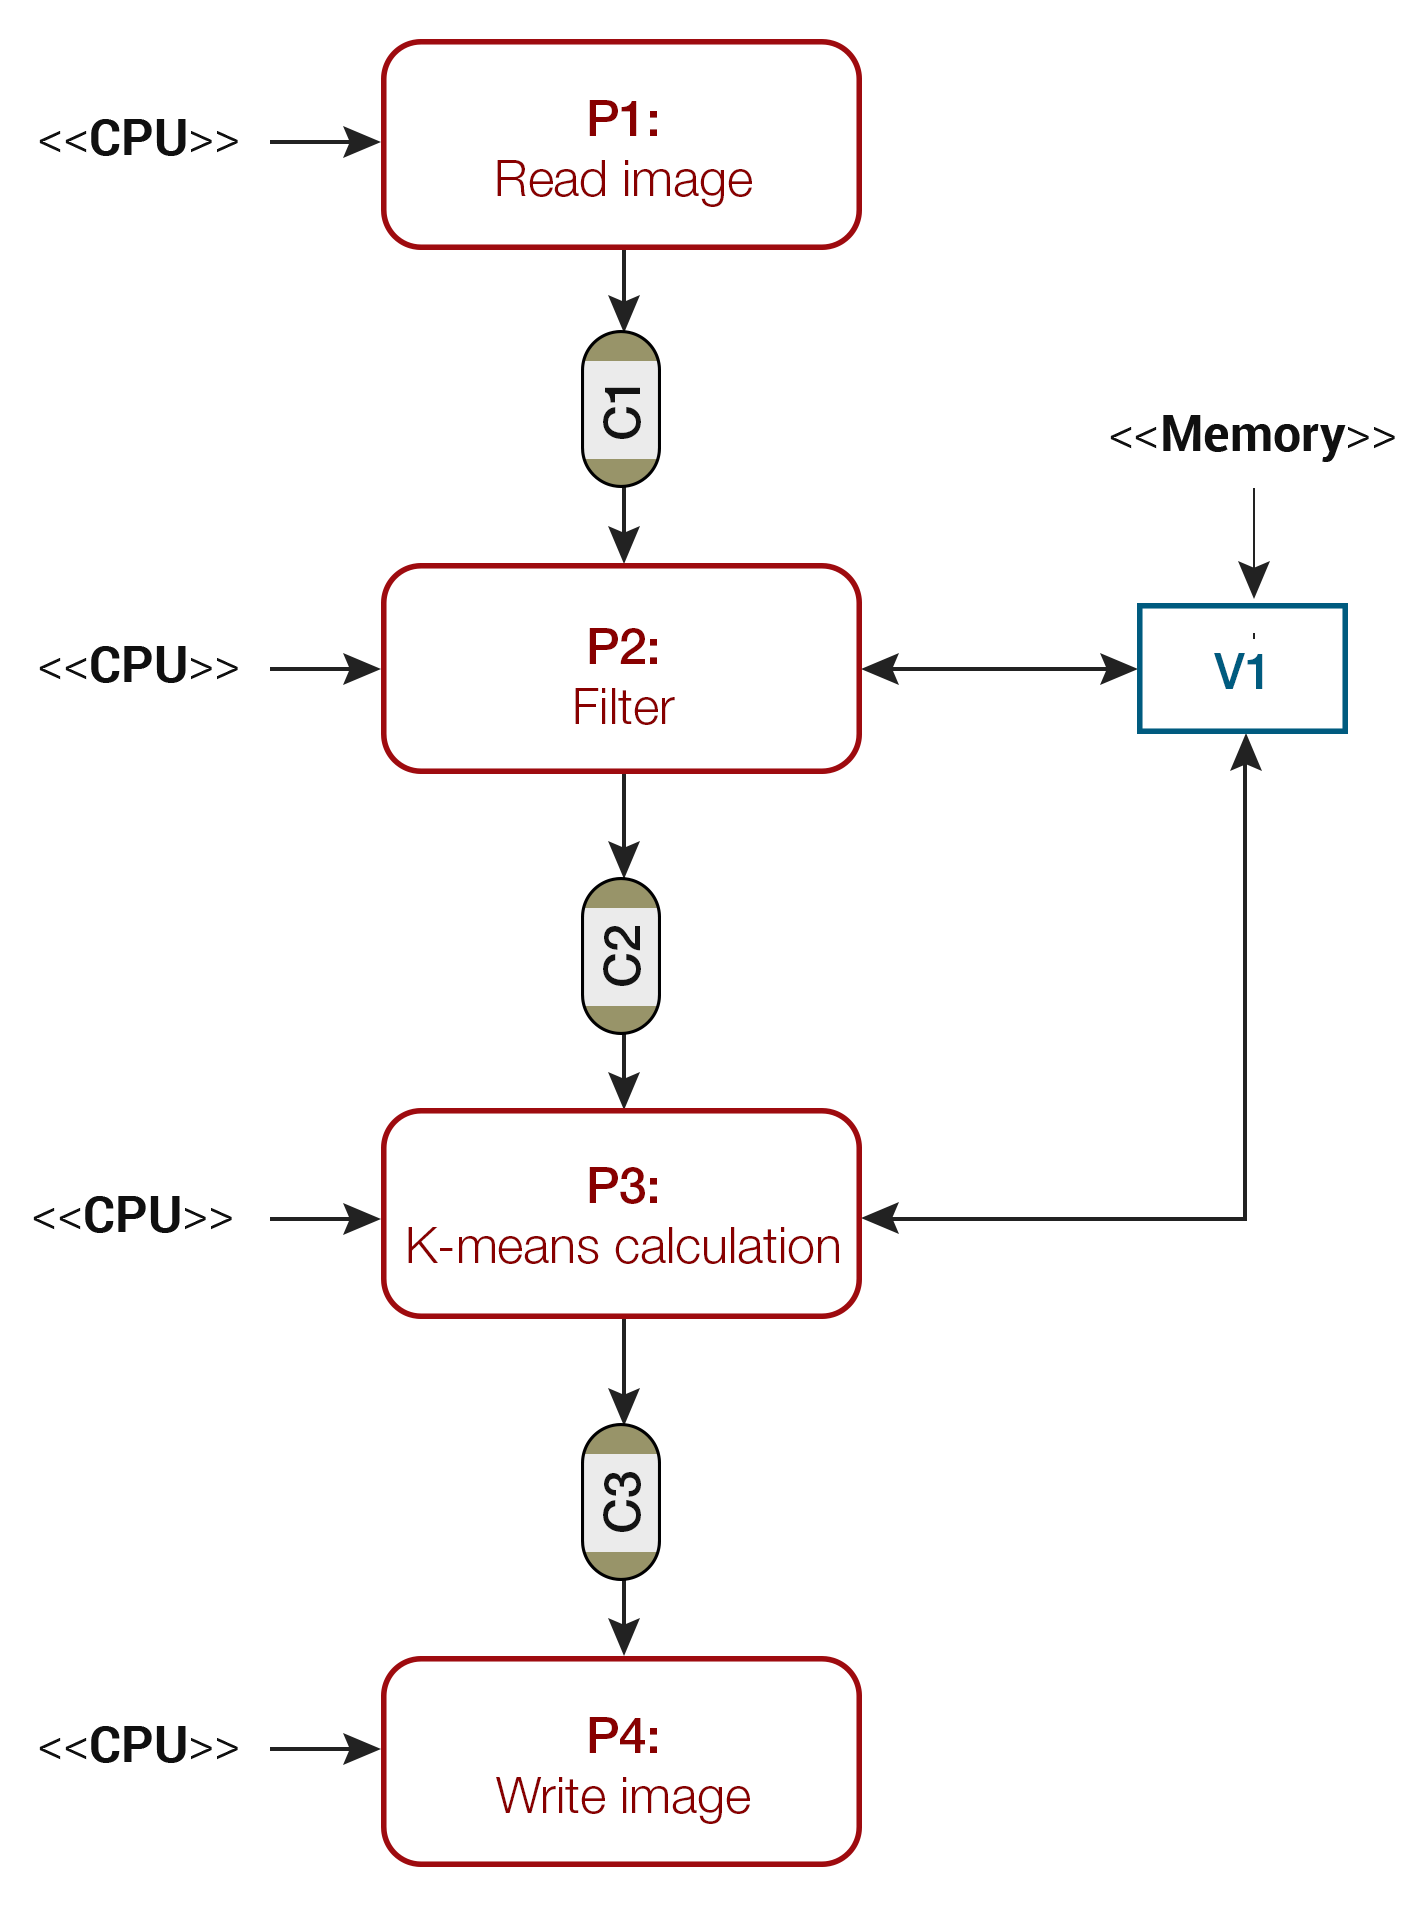
\includegraphics[width = 180 pt]{Binding1}
\caption{1st alternative of binding}
\label{fig:Binding1}
\end{figure}

\begin{figure}[H]
\centering
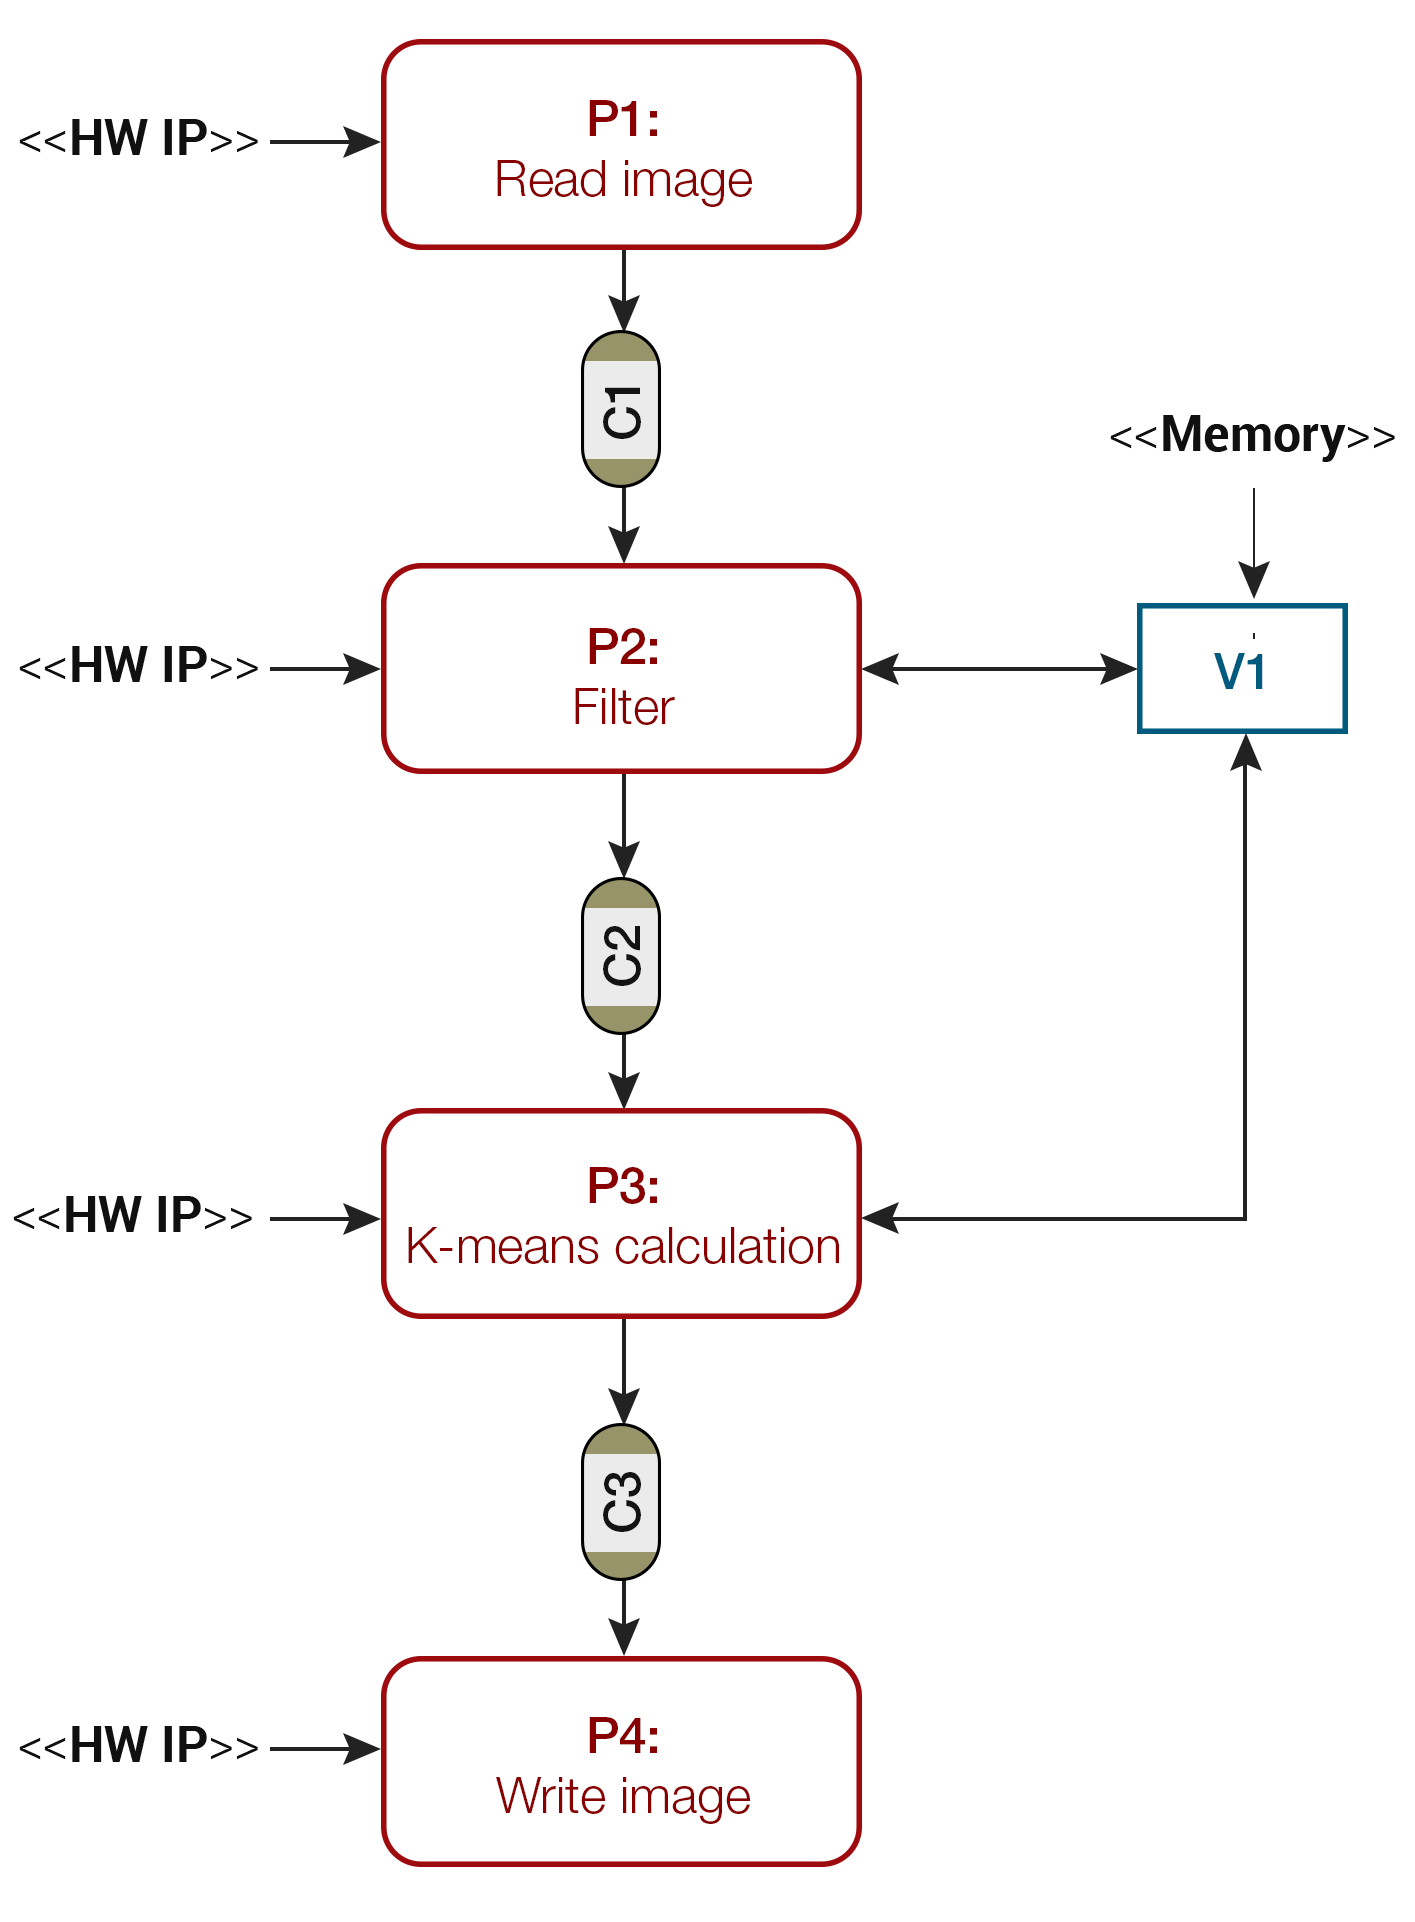
\includegraphics[width = 180 pt]{Binding2}
\caption{2nd alternative of binding}
\label{fig:Binding2}
\end{figure}

\begin{figure}[H]
\centering
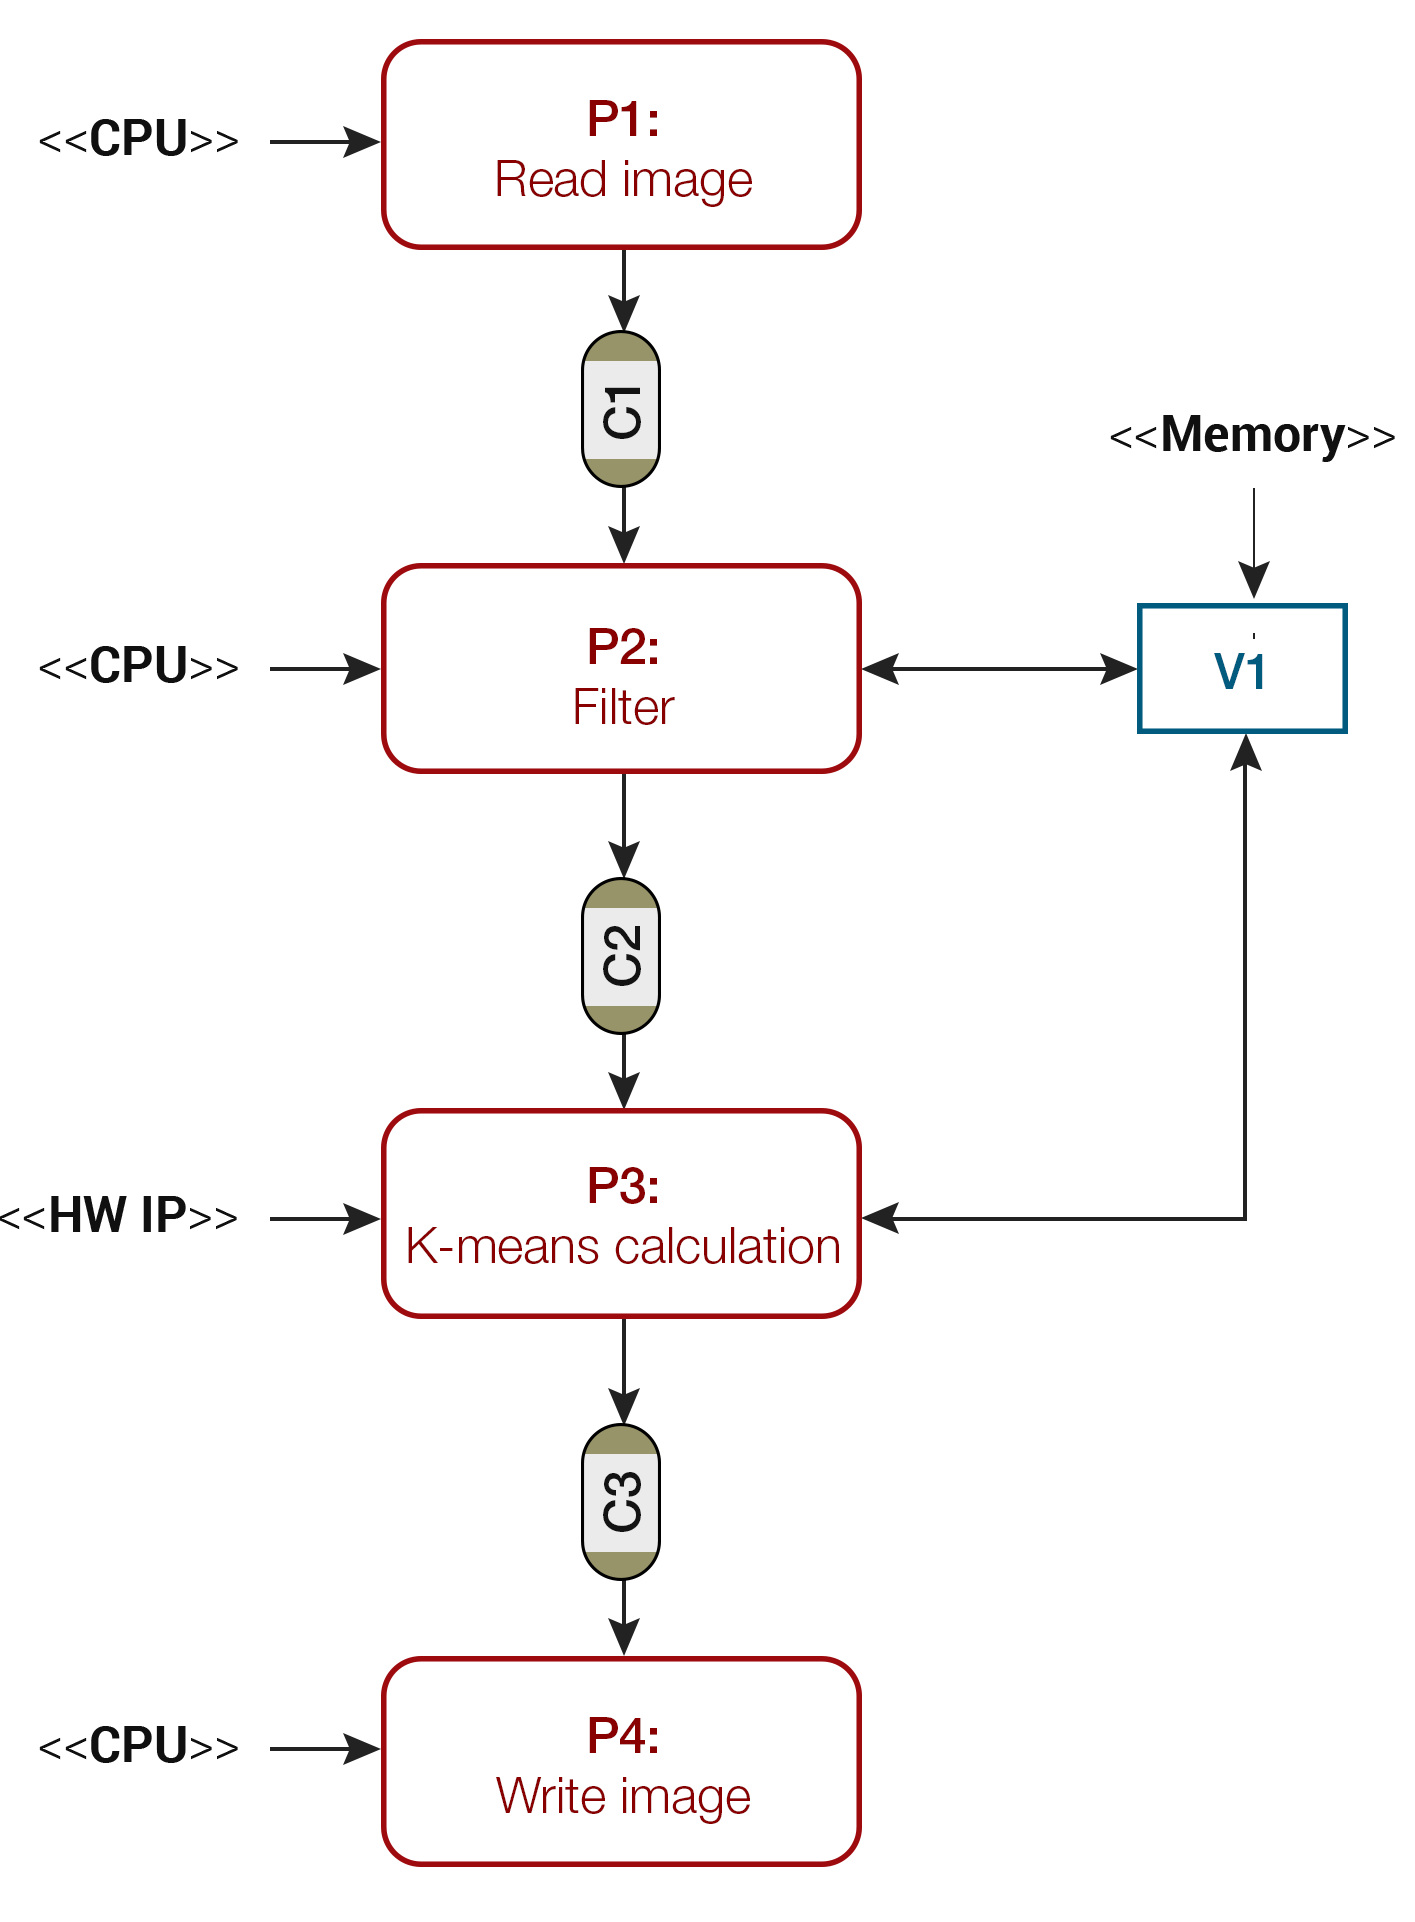
\includegraphics[width = 180 pt]{Binding3}
\caption{3rd alternative of binding}
\label{fig:Binding3}
\end{figure}


\section{Scheduling}